\documentclass{article} 
\usepackage{beamerarticle}

%\documentclass[ignorenonframetext]{beamer} 
%\usetheme{Warsaw}
%\usepackage{lipsum}


\usepackage{hyperref}
\usepackage[references,links]{agda}
\usepackage{amsmath}
\usepackage{amsthm}
\usepackage{mathtools}
\usepackage{textgreek}
\usepackage{catchfilebetweentags}
\usepackage{tipa}
\usepackage{graphicx}
\usepackage{bussproofs}
\usepackage{tikz}
\usepackage{parskip}

%math
\newcommand{\alp}{\ensuremath{\alpha}}
\newcommand{\lamb}{\ensuremath{\lambda}}
\newcommand{\alpsym}{\ensuremath{\sim_\alpha}}
\newcommand{\choice}{\ensuremath{\chi}}
\newcommand{\p}{\ensuremath{\rightrightarrows}}
\newcommand{\pn}{\ensuremath{\rightrightarrows_n}}
\newcommand{\ninb}{\ensuremath{\not\in_b}}
\newcommand{\inb}{\ensuremath{\in_b}}
\newcommand{\bvc}{\textbf{bvc}}

%Agda
\newcommand{\freshin}[2]{\ensuremath{#1 \mathbin{\AgdaDatatype{\#}} #2}}
\newcommand{\lambAg}[2]{\ensuremath{\AgdaInductiveConstructor{ƛ}\, #1\, #2}}
\newcommand{\inAg}{\ensuremath{\mathbin{\AgdaFunction{∈}}}}
\newcommand{\ninAg}{\ensuremath{\mathbin{\AgdaFunction{∉}}}}
\newcommand{\neqAg}{\ensuremath{\mathbin{\AgdaInductiveConstructor{≢}}}}
\newcommand{\ap}[2]{#1 \ensuremath{\mathbin{\AgdaInductiveConstructorFunction{·}} #2}}
\newcommand{\var}[1]{\ensuremath{\AgdaInductiveConstructorFunction{v}\, #1}}
\newcommand{\fv}{\ensuremath{{\AgdaFunction{fv}}\,}}
\newcommand{\perm}{\ensuremath{\mathbin{\AgdaFunction{∙}}}}
\newcommand{\perma}{\ensuremath{\mathbin{\AgdaFunction{∙}_a}}}
\newcommand{\free}{\ensuremath{\mathbin{\AgdaFunction{*}}}}
\newcommand{\choiceAg}{\ensuremath{\AgdaFunction{χ}\,}}
\newcommand{\choiceAgaux}{\ensuremath{\AgdaFunction{χ'}\,}}
\newcommand{\alpeqAg}{\ensuremath{\mathbin{\AgdaDatatype{∼α}}}}
\newcommand{\swap}[3]{\ensuremath{(#1 \mathbin{\AgdaFunction{∙}} #2)\, #3}}
\newcommand{\betar}{\ensuremath{\rightarrow_{\beta}}}
\newcommand{\betarn}{\ensuremath{\rightarrow_{\beta n}}}
\newcommand{\betaalpha}{\ensuremath{\rightarrow_\alpha}}
\newcommand{\f}{\ensuremath{\rightarrow}}
\newcommand{\betaaster}{\ensuremath{\rightarrow_\beta^*}}
\newcommand{\lam}{\ensuremath{\lambda}}
\newcommand{\conc}{\ensuremath{\mathop{+\!\!+}}}


% \newcommand{\agdaf}[1]{\ensuremath{\AgdaFunction{#1}\,}}
% \newcommand{\agdaD}[1]{\ensuremath{\AgdaDatatype{#1}\,}}
% \newcommand{\agdav}[1]{\ensuremath{\AgdaBound{#1}\,}}

\DeclareUnicodeCharacter{411}{\textipa{\textcrlambda}}
\DeclareUnicodeCharacter{65288}{(}
\DeclareUnicodeCharacter{65289}{)}
\DeclareUnicodeCharacter{8788}{\ensuremath{\coloneqq}}
\DeclareUnicodeCharacter{8336}{\ensuremath{_a}}
\DeclareUnicodeCharacter{8799}{\ensuremath{\overset{?}{=}}}
\DeclareUnicodeCharacter{8759}{\ensuremath{\dblcolon}}
\DeclareUnicodeCharacter{8718}{\ensuremath{\square}}

\newtheorem{lem}{Lemma}

\title{Parallel Reduction}

\begin{document}
\maketitle

\section{Barendregt BVC Convention}

Next we extract from page 26 of~\cite{barendregt81} the following variable convention and definitions.

\subsubsection*{2.1.12 Convention}

Terms that are \alp-congruent are identified.

\subsubsection*{2.1.13 Variable Convention}

If $M_1, \dots M_n$ occur in certain mathematical context, then in these terms all bound variables are chosen to be different from the free variables.


\subsubsection*{2.1.12 Substitution Definition} \label{sec:substitutionBarendregt}

\[
  \begin{array}{llcll}
    x &[x:=N] & \equiv & N &\\
    y &[x:=N] & \equiv & y & \text{if}\ x \not\equiv y\\
    (M_1 M_2) &[x:=N]& \equiv & (M_1 [x:=N]) (M_2 [x:=N]) &\\
    (\lam y . M_1) & [x:=N] & \equiv & \lam y . (M_1 [x:=N])&\\
  \end{array}
\]

\label{notefourth} In the fourth clause it is not needed to say ``provided that $y \not\equiv x$\ and $y \not\in fv(N)$''. By the variable convention this is the case.

There exist subtleties in the use of variable convention. We show next one example of these caused by the composite use of it in the following results.


\subsubsection*{2.1.16 Substitution Composition Lemma}

If $x \not\equiv y$\ and $x \not\in fv(L)$ then:

\[ M [x:=N][y:=L] \equiv M[y:=L][x:=N[y:=L]] \]

Proof: By induction on $M$.
\begin{itemize}
\item{Case 1} $M$ is a variable.
  \begin{itemize}
  \item{Sub-Case 1.2} $M \equiv y$. Then both sides equal L, for $x \not\in fv(L)$ implies $L[x:=N]\equiv L$.
    To prove $x \not\in fv(L)$ implies $L[x:=\dots]\equiv L$\ we need to make use of the variable convention with context $x,L,N$, by doing so we get that $x \ninb L$. Next we show that this premise is necessary in the abstraction case of an induction over $L$.

\begin{itemize}
\item Abstraction case $L = \lam y . M$.  We have to prove that $x \not\in fv(\lam y . M) \Rightarrow (\lam y . M)[ x := N] \equiv \lam y . M$.
  \[\begin{array}{ll}
      (\lam y . M)[ x := N] & \equiv \text{by BVC } y \not\equiv x \text{ and } y \not\in fv(N) \\
      \lam y . (M [ x := N]) & \equiv \text{by i.h. using } x \not\in fv(M) \text{ as } y \not\equiv x \\
      \lam y . M
  \end{array}\]
\end{itemize}

  \end{itemize}
\item{Case 2} $M \equiv \lamb z . M_1$. Again using BVC we may assume that $z \not\equiv x$\ and $z \not\in fv(N,L)$.
\[ \begin{array}{rl}
     (\lam z. M_1)[x:=N][y:=L]      & \equiv  \{z \not\equiv x, y \text{ and } z \not\in fv(N,L) \} \\
     \lam z . M_1[x:=N][y:=L]       & \equiv  \{\text{i.h. as } x \not\equiv y, x \not\in fv(L) \} \\
     \lam z . M_1[y:=L][x:=N[y:=L]] & \equiv  \\
     (\lam z . M_1) [y:=L][x:=N[y:=L]] & \\
  \end{array}\]

  So we need the BVC convention holds under the context $x,y,M,N,L$\ in this sub-case.
\end{itemize}


We can conclude, recollecting the uses of BVC from previous proof sub-cases, that substitution composition lemma needs that the BVC hold in the context of $x,y,M,N,L$.

Previous result is used inside the 1.2 sub-case of substitution composition lemma proof (page 60 of~\cite{barendregt81}). We show that the freshness context of previous result can not be obtained inside the proof of the next result.

\subsubsection*{3.2.4 Substitution preserves parallel relation.}

      \[ M \p M' , N \p N' \Rightarrow M [x:=N] \p M'[x:=N'] \]

By induction on the relation, we show the following problematic sub-case.

\begin{itemize}
\item{Case 4.} $M \p M' \equiv (\lam y. P)Q \p P'[y:=Q']$\ as a direct consequence of $P \p P'$, $Q \p Q'$.
  \[\begin{array}{ll}
      ((\lam y. P)Q) [x:=N] & \equiv \text{by BVC } y \not\equiv x \text{ and } y \not\in fv(N) \\
      (\lam y. (P [x:=N]))(Q [x:=N])  & \p \text{by i.h. and applying } \pn \beta\} \\
      P'[x:=N'][y := Q'[x:=N']  & \equiv \text{by lemma 2.1.16} \\
      P'[y:=Q'][x:=N']
  \end{array}\]
\end{itemize}

The first use of BVC can be obtained requiring as BVC context $x,N,M$. But substitution composition lemma needs $y,x,P',Q',N'$ as BVC context. The $x,P',Q',N'$\ context could be derived from $x,M,N$ context, as parallel reduction does not create bound neither free variables, thus BVC is preserved, but $y$ is a bound variable of $M$ and so we can not put it in the BVC context of this proof. This problematic use of BVC can not be easily fixed. A fresh variable rename can be done, using that \alp-congruent terms are identified, but then, as we are in a relation induction, the inductive hypothesis will not hold over the renamed sub-term. Thus, this proof can not be fixed in a simple manner. Furthermore, an induction on terms, or even in the length of terms, can not be done because of the $M \p M$\ introduction rule of parallel relation definition. 

We propouse a solution to this problem, adding to the BVC convention that all bound variables are distinct. By doing so we can know that the bound variable $y$\ does not occur bind in the context $x,P',Q',N'$, and thus the free variables will not occur bind in the BVC context $y,x,P',Q',N'$\ as needed inside the previous proof sub-case.

In~\cite{hindley:2008}, Hindley suggests in lemma 1.20 that we can work removing BVC precondition and replacing term's identity by \alp-equivalence relation, and all theorems will stay true. This work follow this idea up to the diamond property of parallel reduction, crux result for the Church-Rosser theorem. In the next section we justify our variation of the BVC in a more general way. Then, we prove several classic results assuming the proposed variaton of the BVC convention. Our proofs will follow common practice in classic pen-and-paper theory, but adding special attention to the required freshness premises contexts. Finally, we will remove the variable convention premise to prove the confluence of the parallel reduction relation.

\section{New Variable Convention (NVC)}

As in the BVC, if $M_1, \dots M_n$ occur in certain mathematical context, then in these terms all bound variables are chosen to be different all different between them, and also different from the free variables. As previously said, we add that all bound variables must be different. We already explained this addition in the context of a particular proof in previous section. But now we will try to give the intuition behind this addition, justiying its neccessary in a more general way.

To reason as in informal practice, the BVC convention should be preserved over terms and relations inductions, to be able to correctly apply the inductive hypotheses under valid freshness premises. We show that this is not the case for the BVC, as it is not preserved in the abstraction case of an induction over terms. That is, with premise $fv (\lam x. M) \ninb \lam x .M$\ we need to prove that $fv(M) \ninb M$. By free variables definition: $fv (M) - \{ x \}  \ninb \lam x .M$, thus using $\ninb$\ definition, $fv (M) - \{ x \}  \ninb M$. In the case that $x \in fv(M)$, we can not get the desired result because we can not infer $x \ninb M$. However, if we assume all bound are not equal in $\lam x . M$, then $x \ninb M$\ follows directly.

Another important difference with the BVC convention is that we will not identify \alp-compatible terms in our work.

\section{Parallel Reduction}\label{parallel}

We introduce the naive parallel reduction relation, almost identical to Barendregt ones, but replacing $M \p M$\ rule with $x \p x$\ one. Note that the naive substitution is used in the last rule, implemented as a direct fold and equivalent to Barendregt's substitution definition previously introduced in~\ref{sec:substitutionBarendregt}.

\begin{minipage}{0.25\linewidth}
  \AxiomC{$$}   \LeftLabel{\pn v} \UnaryInfC{$x \pn x$} \DisplayProof
\end{minipage}
\begin{minipage}{0.45\linewidth}
  \AxiomC{$M \pn M'$} 
  \AxiomC{$N \pn N'$}
  \LeftLabel{\pn a}
  \BinaryInfC{$M N \pn M' N'$} \DisplayProof
\end{minipage}
\begin{minipage}{0.25\linewidth}
  \AxiomC{$ M \pn N$} 
  \LeftLabel{\pn \lam}
  \UnaryInfC{$\lambda x M  \pn  \lambda x N$} \DisplayProof
\end{minipage}

\begin{center}
  \AxiomC{$M \pn M'$}
  \AxiomC{$N \pn  N'$}
  \LeftLabel{$\pn \beta$}
  \BinaryInfC{$(\lambda x M) N  \pn M' [x := N']_n$}
  \DisplayProof
\end{center}

We can prove substitution composition lemma 3.2.4 in a similar way to Barendregt work, under the hypothesis of the NVC variable convention.

Following Takahashi~\cite{TAKAHASHI1995120} work to prove the confluence property of the parallel relation, we define the aster function that recursively reduces all $\beta$-redexes in a term.

  \[
  \begin{array}{llll}
    x &&^* &= x \\
    (\lam x . M)&&^* &= \lam x . M^* \\
    (x &M)&^* &= x M^*  \\
    ((M_1 M_2) & M_3)&^* &= (M_1 M_2)^* M_3^* \\
    ((\lam x . M_1) & M_2)&^* &= M_1^* [x := M_2^*]_n 
  \end{array} 
  \]
  
  Using the substitution composition lemma we can prove next lemma.

  \begin{lemma}$NVC\ M, M \pn N \Rightarrow N \pn M^*$ 
  \end{lemma} \label{lemma:aster}
  \begin{proof}
   The proof is by a  direct induction on term $M$, except from the next application sub-case.

  \begin{itemize}
  \item{Application $M \equiv (\lam x . M) N$, $\pn \beta$\ sub-case. }

    \begin{minipage}{0.5\linewidth}
    Hypotheses:
      \AxiomC{$M \pn M'$}
      \AxiomC{$N \pn  N'$}
      \LeftLabel{$\pn \beta$}
      \BinaryInfC{$(\lambda x M) N  \pn M' [x := N']_n$}
      \DisplayProof
  \end{minipage}
  \begin{minipage}{0.5\linewidth}
    Thesis: \[ M' [x := N']_n \pn  \underbrace{((\lambda x M) N)^*}_{=M^* [x := N^*]_n}\]
  \end{minipage}
  Proof:
  \AxiomC{$M \pn M'$}
  \LeftLabel{ih}
  \UnaryInfC{$M' \pn M^*$}
  \AxiomC{$N \pn  N'$}
  \LeftLabel{ih}
  \UnaryInfC{$N' \pn N^*$}
  \LeftLabel{lem. 3.2.4}
  \BinaryInfC{$M' [x := N']_n \pn  M^* [x := N^*]_n$}
  \DisplayProof


  
  The application of lemma 3.2.4 in previous proof tree requires the NVC context $x,M',N'$, which can be derived from knowing NVC holds for $(\lambda x M) N$\ and that \pn\ relation preserves the NVC convention. Again, here is essential that all binder are different in the NVC context.
\end{itemize}
    
  \end{proof}

From this result it is directly derived that \pn\ has diamond property. Also we can prove it is preserved under variable swapping operation by a simple term induction.

\begin{theorem}{\pn\ has diamond property}

  \begin{minipage}{0.7\linewidth}
  \[ M \pn N, M \pn P \Rightarrow \exists R, N \pn R, P \pn R \]
\end{minipage}
  \begin{minipage}{0.3\linewidth}
  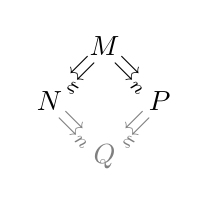
\begin{tikzpicture}[>=latex]
   \node (M) at (0.7,0.7) {$M$};
   \node (N) at (0,0) {$N$};
   \node (P) at (1.4,0) {$P$};
   \node[opacity=0.5] (Q) at (0.7,-0.7) {$Q$};

   \path               (M) --node[sloped ]{\reflectbox{\pn}} (N);
   \path               (M) --node[sloped, auto=false, allow upside down]{\pn} (P) ;
   \path [opacity=0.5] (N) --node[sloped, auto=false, allow upside down]{\pn} (Q);
   \path [opacity=0.5] (P) --node[sloped ]{\reflectbox{\pn}} (Q);
\end{tikzpicture}
\end{minipage}

\end{theorem}\label{theorem:parallelnaive}

\begin{proof}
  Using lemma~\ref{lemma:aster} with both hypotheses we get that $N$\ and $P$ are confluent to $M^*$ in one step of the \pn\ relation.
\end{proof}

Next lemma establish that the introduced relation is independent from variable binders choices, under NVC conditions to ensure that the naive substitution can be correctly applied inside $\pn\beta$ relation rule. In other words, this lemma says that every parallel reduction can be reproduced for any \alp-equivalent term  satisfing the NVC condition.

\begin{lemma}{Naive parallel reduction can be reproduced for NVC \alp-equivalent terms.} \label{lemma:parallelrenaming}


  \[ NVC\ M, NVC\ M', M \pn N \Rightarrow \exists N', N  \alpsym N', M' \pn N' \]
  \begin{center}
  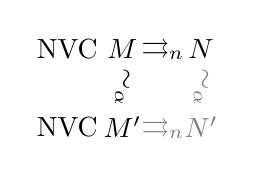
\begin{tikzpicture}[>=latex]
   \node (M) at (0,1) {$M$};
   \node (NVCM) at (-0.7,1) {NVC};
   \node (M') at (0,0) {$M'$};
   \node (NVCM') at (-0.7,0) {NVC};
   \node (N) at (1,1) {$N$};
   \node[opacity=0.5] (N') at (1,0) {$N'$};

   \path               (M) --node{\pn} (N);
   \path [opacity=0.5,->] (M') --node{\pn} (N') ;
   \path               (M) --node[sloped]{$\alpsym$} (M');
   \path [opacity=0.5] (N) --node[sloped]{$\alpsym$} (N');
\end{tikzpicture}
  \end{center}

\end{lemma}

\begin{proof} By induction over the term $M$.

  \begin{itemize}
  \item{Variable case. $M = x$ is direct.}
  \item{Application case. $M = (\lambda x . M) N$}
    \begin{itemize}
    \item{$\pn$a sub-case. Direct.}

    \item{$\pn\beta$\ sub-case.}
      
      Hypotheses: The NVC conditions holds for terms $(\lambda x . M) N$\ and $(\lambda y . P) Q$.
      \begin{center}

      \AxiomC{$M \pn M'$}
      \AxiomC{$N \pn  N'$}
      \LeftLabel{$\pn \beta$}
      \BinaryInfC{$(\lambda x. M) N  \pn M' [x := N']_n$}
      \DisplayProof

      \AxiomC{$\lam x .M \alpsym \lam y. P$}
      \AxiomC{$N \alpsym  Q$}
      \LeftLabel{$\alpsym \cdot$}
      \BinaryInfC{$(\lambda x .M) N \alpsym (\lambda y. P) Q$}
      \DisplayProof
      \end{center}

      Thesis: $\exists R, (\lambda y .P) Q \pn R, M' [x := N']_n \alpsym R$
      
      We can apply the inductive hypothesis to $N$.

      \begin{center}
        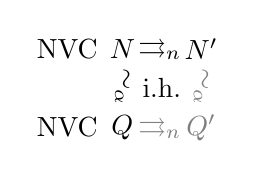
\begin{tikzpicture}[>=latex]
          \node (N) at (0,1) {$N$};
          \node (hi) at (0.5,0.5) {i.h.};
          \node  (NVCN) at (-0.7,1) {NVC};
          \node  (Q) at (0,0) {$Q$};
          \node  (NVCQ) at (-0.7,0) {NVC};
          \node (N') at (1,1) {$N'$};
          \node[opacity=0.5] (Q') at (1,0) {$Q'$};
          
          \path               (N) --node{\pn} (N');
          \path [opacity=0.5] (Q) --node{\pn} (Q') ;
          \path  (N) --node[sloped]{$\alpsym$} (Q);
          \path [opacity=0.5] (N') --node[sloped]{$\alpsym$} (Q');
        \end{tikzpicture}
      \end{center}
      
      We can derive $M \alpsym (y\ x) P$ from $\lam x . M \alpsym \lam y . P$. Then, as we know that NVC condition is preserved through term induction, NVC holds for $P$, and as NVC is equivariant, NVC also holds for $(y\ x) P$. We can now apply the inductive hypothesis to $M$ and get:

    \begin{center}
      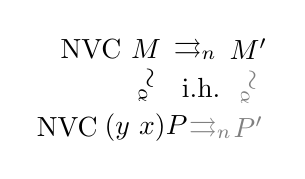
\begin{tikzpicture}[>=latex]
   \node (M) at (0,1) {$M$};
   \node (hi) at (0.7,0.5) {i.h.};
   \node  (NVCN) at (-0.7,1) {NVC};
   \node  (P) at (0,0) {$(y\ x) P$};
   \node  (NVCQ) at (-1,0) {NVC};
   \node (M') at (1.3,1) {$M'$};
   \node[opacity=0.5] (P') at (1.3,0) {$P'$};

   \path               (M) --node{\pn} (M');
   \path [opacity=0.5] (P) --node{\pn} (P') ;
   \path  (M) --node[sloped]{$\alpsym$} (P);
   \path [opacity=0.5] (M') --node[sloped]{$\alpsym$} (P');
 \end{tikzpicture}
\end{center}
    
   We can reason reason as follows:

   \begin{center}
   \AxiomC{$(y\ x) P \pn P'$}
   \LeftLabel{\pn is equiv.}
   \UnaryInfC{$P \pn (y\ x) P'$}
   \AxiomC{$Q \pn Q'$}
   \LeftLabel{$\pn\beta$}
   \BinaryInfC{$(\lam y .P) Q \pn ((y\ x) P')[y:=Q']_n$}
   \DisplayProof
   \end{center}

   We end the prove by proving that $((y\ x) P')[y:=Q']_n$ is the $R$ term satisfing the thesis. For this, it only remains to be proved that $M'[x:=N']_n \alpsym ((y\ x) P')[y:=Q']_n$, which we derive next.

\[ \begin{array}{rcl}
     ((y\ x) P') &[y:=Q']_n  &\alpsym \{ \text{naive subst. lem.} \}\\
     ((y\ x) P') &[y:=Q']    &\equiv\  \{ \text{lem.} \} \\
     P'          &[x:=Q']    &\alpsym \{ \text{subst. lem., as } P'\alpsym M', Q' \alpsym N' \}\\
     M'          &[x:=N']    &\alpsym \{ \text{naive subst. lem.} \}\\
     M'          &[x:=N']_n 
   \end{array}\]
   
   The first application of the naive substitution lemma in previous derivation requires $y \ninb (y\ x) P'$\ and $fv(Q') \ninb (y\ x) P'$. As the parallel reduction does not introduce binders, from  $y \ninb P$\ and $P \pn (y\ x) P'$\ we can directly derive $y \ninb (y\ x) P'$.  Whereas, we can check $fv(Q') \ninb (y\ x) P'$\ in the following way; as parallel reduction does not introduce free variables and $Q \pn Q'$, we get $fv(Q') \subseteq fv(Q)$. By hypotheses $fv(Q) \ninb P$, thus using previous result, $fv(Q') \ninb P$, from which using that parallel reduction does not intruduce binders and $P \pn (y\ x) P'$, we can conclude $fv(Q') \ninb (y\ x) P'$. The second naive substitutuion lemma application needs as premises: $x \ninb M'$\ and $fv(N') \ninb M'$, which can be derived in a similar way.
   
 \end{itemize}

\item{Abstraction case. $M = \lambda x . M$}

Hypotheses:
\begin{minipage}{0.3\linewidth}
  \AxiomC{$ M \pn N$} 
  \LeftLabel{\pn \lam}
  \UnaryInfC{$\lambda x . M  \pn  \lambda x. N$} \DisplayProof
\end{minipage}
\begin{minipage}{0.3\linewidth}
  , $\lambda x . M  \alpsym  \lambda y . N$
\end{minipage}

Thesis: $\exists R, \lam y . N \pn R, \lam x . N \alpsym R$

We can derive $M \alpsym (y\ x) N$\ from $\lambda x.  M  \alpsym  \lambda y. N$, then we can apply the inductive hypothesis as NVC is equivariant, so NVC also holds in $(y\ x) N$.

    \begin{center}
      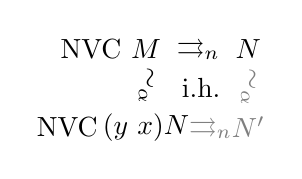
\begin{tikzpicture}[>=latex]
   \node (M) at (0,1) {$M$};
   \node (hi) at (0.7,0.5) {i.h.};
   \node  (NVCN) at (-0.7,1) {NVC};
   \node  (P) at (0,0) {$(y\ x) N$};
   \node  (NVCQ) at (-1,0) {NVC};
   \node (N) at (1.3,1) {$N$};
   \node[opacity=0.5] (N') at (1.3,0) {$N'$};

   \path               (M) --node{\pn} (N);
   \path [opacity=0.5] (P) --node{\pn} (N') ;
   \path  (M) --node[sloped]{$\alpsym$} (P);
   \path [opacity=0.5] (N) --node[sloped]{$\alpsym$} (N');
 \end{tikzpicture}
\end{center}

  As parallel relation is equivariant we can derive $N \pn (y\ x) N'$, from which by $\pn\lam$ rule we get $\lam y. N \pn \lam y . ((y\ x) N')$. This last term is the $R$ we are looking for in the thesis, we just need to prove that is \alp-compatible with $\lam x . N$, which can be derive as follows:

\[
\begin{array}{rcl}
  \lam y . ((y\ x) N') &\alpsym & \{ \text{as } y \# N' \vee x = y \} \\
  \lam x .  N' &\alpsym & \{ \text{as } N \alpsym N' \} \\
  \lam x . N
\end{array}
\]

The fresh premise in previous derivation can be derived if $x \not= y$ in the next way, trivally $x \# \lam x .M$, then $x \# \lam y . N$\ as $\lam x . M \alpsym \lam y . N$. Then, as $x \not= y$, $x \# N$ from which $y \# (y\ x) N$. By variable freshness preservation under parallel reduction and from $(y\ x) N \pn N'$\ holds we infer that $y \# N'$\ holds.

\end{itemize}
   
\end{proof}

As we do not identify \alp-compatible terms, as the BVC convention does, we need to introduce the correct parallel relation definition, which works over the entire set of terms, that is without assuming we work only with NVC terms. Then, we will prove that the introduced relation works in fact over \alp-equivalence classes of terms. Finally, we prove the diamond property of this relation.

\begin{definition}{Parallel Reduction}

\[ M \p N \equiv \exists M',N', NVC\ M', M \alpsym M', M' \pn N' , N' \alpsym N \]

\begin{center}
  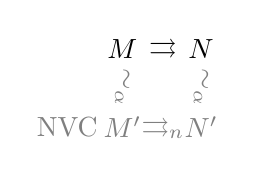
\begin{tikzpicture}[>=latex]
   \node (M) at (0,1) {$M$};
   \node [opacity=0.5] (M') at (0,0) {$M'$};
   \node [opacity=0.5] (NVC) at (-0.7,0) {NVC};
   \node (N) at               (1,1) {$N$};
   \node[opacity=0.5] (N') at (1,0) {$N'$};

   \path               (M) --node{\p} (N);
   \path [opacity=0.5] (M') --node{\pn} (N') ;
   \path [opacity=0.5] (M) --node[sloped]{$\alpsym$} (M');
   \path [opacity=0.5] (N) --node[sloped]{$\alpsym$} (N');
\end{tikzpicture}
\end{center}

\end{definition}

This relation trivally preserved by \alp-conversion and swapping operation. Now we prove the diamond property of \p.

\begin{theorem}{\p\ has diamond property}

  \begin{minipage}{0.7\linewidth}
  \[ M \p N, M \p P \Rightarrow \exists R, N \p R, P \p R \]
\end{minipage}
  \begin{minipage}{0.3\linewidth}
  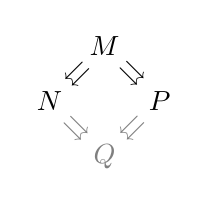
\begin{tikzpicture}[>=latex]
   \node (M) at (0.7,0.7) {$M$};
   \node (N) at (0,0) {$N$};
   \node (P) at (1.4,0) {$P$};
   \node[opacity=0.5] (Q) at (0.7,-0.7) {$Q$};

   \path               (M) --node[sloped, auto=false, allow upside down]{\p} (N);
   \path               (M) --node[sloped, auto=false, allow upside down]{\p} (P) ;
   \path [opacity=0.5] (N) --node[sloped, auto=false, allow upside down]{\p} (Q);
   \path [opacity=0.5] (P) --node[sloped, auto=false, allow upside down]{\p} (Q);
\end{tikzpicture}
\end{minipage}

\end{theorem}

\begin{proof}
  Hypotheses: 


    \begin{align}
    M \p N \equiv \exists M', N', NVC\ M', M \alpsym M', M' \pn N' , N' \alpsym N \label{theorem:confluencehi1}\\
    M \p P \equiv \exists M'',P', NVC\ M'', M \alpsym M'' ,M'' \pn P',  P' \alpsym P \label{theorem:confluencehi2}
      \end{align}\label{theorem:confluence}
      \begin{center}
  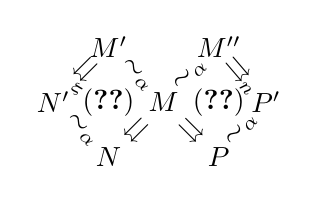
\begin{tikzpicture}[>=latex]

   \node (M'') at (1.4,1.4) {$M''$};    
   \node (M') at (0,1.4) {$M'$};
   \node (M) at (0.7,0.7) {$M$};
   \node (1) at (0,0.7) {$(\ref{theorem:confluencehi1})$};
   \node (2) at (1.4,0.7) {$(\ref{theorem:confluencehi2})$};
   \node (N) at (0,0) {$N$};

   \node (N') at (-0.7,0.7) {$N'$};
   \node (P) at (1.4,0) {$P$};
   \node (P') at (2,0.7) {$P'$};

   \path               (M') --node[sloped]{\alpsym} (M);
   \path               (N) --node[sloped]{\alpsym} (N');
   \path               (M'') --node[sloped]{\alpsym} (M);
   \path               (P) --node[sloped]{\alpsym} (P');

   \path               (M'') --node[sloped]{\pn} (P');
   \path               (M) --node[sloped,  allow upside down]{\p} (N);
   \path               (M') --node[sloped]{\reflectbox{\pn}} (N');
   \path               (M) --node[sloped, auto=false, allow upside down]{\p} (P) ;
 \end{tikzpicture}
      \end{center}

The proof follows next figure sketch. First, as NVC holds for $M'$\ and $M''$, by lemma~\ref{lemma:parallelrenaming} there exist $N''$\ such that $N' \alpsym N''$\ and $M'' \pn N''$. As \pn\ preserves NVC convention, using the diamond property of \pn (theorem~\ref{theorem:parallelnaive}) we know that $N''$\ and $P'$ are confluent terms applying one step of \pn\ relation to some term $Q$. Finally, $N$\ and $P$\ are also confluent terms by \p\ definition.
      
      \begin{center}
        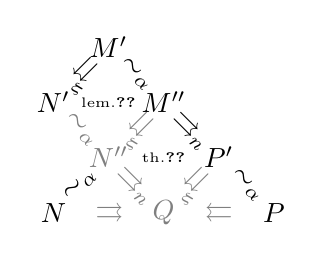
\begin{tikzpicture}[>=latex]

          \node (M') at (0,1.4) {$M'$};
          \node (M'') at (0.7,0.7) {$M''$};
          \node [opacity=0.5] (N'') at (0,0) {$N''$};
          \node [opacity=0.5] (Q) at (0.7,-0.7) {$Q$};
          \node (N') at (-0.7,0.7) {$N'$};
          \node (1) at (0,0.7) {{\tiny lem.\ref{lemma:parallelrenaming}}};
          \node (P') at (1.4,0) {$P'$};
          \node (N) at (-0.7,-0.7) {$N$};
          \node (P) at (2.1,-0.7) {$P$};
          \node  (2) at (0.7,0) {{\tiny th.\ref{theorem:parallelnaive}}};

          \path               (N) --node[sloped]{\alpsym} (N'');
          \path               (P) --node[sloped]{\alpsym} (P');
          \path               (M') --node[sloped]{\alpsym} (M'');
          \path [opacity=0.5] (N') --node[sloped]{\alpsym} (N'');
          \path               (M') --node[sloped]{\reflectbox{\pn}} (N');
          \path [opacity=0.5] (M'') --node[sloped]{\reflectbox{\pn}} (N'');
          \path [opacity=0.5] (N'') --node[sloped]{\pn} (Q);
          \path [opacity=0.5] (P') --node[sloped]{\reflectbox{\pn}} (Q);
          \path               (M'') --node[sloped]{\pn} (P');
          \path [opacity=0.5] (N) --node[sloped]{\p} (Q);
          \path [opacity=0.5] (P) --node[sloped]{\reflectbox{\p}} (Q);
        \end{tikzpicture}
      \end{center}
\end{proof}


We now introduce the $\beta$-reduction relation, similar to previously done withe the parallel reduction definition, we first inductively define the naive definitions, based on the naive subtitution operation, and then based on them the proper ones. The naive $\beta$-reduction relation \betarn\ is defined as the contextual clousure of the following $\beta$-contraction relation as usual. 

\begin{definition}{Naive $\beta$-contraction}
    \[ (\lam x . M) N \triangleright M [ x:= N ]_n \]
\end{definition}

Next, we define the $\beta$-reduction relation over the real calculus.

\begin{definition}{$\beta$-reduction}
    \[ M \betar N \equiv \exists M',N', M \alpsym M', N \alpsym N', BVC\ M', M' \betarn N'  \]

\begin{center}
  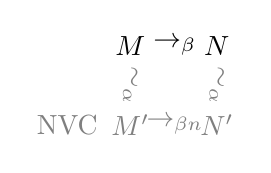
\begin{tikzpicture}[>=latex]
   \node (M) at (0,1) {$M$};
   \node [opacity=0.5] (M') at (0,0) {$M'$};
   \node [opacity=0.5] (NVC) at (-0.8,0) {NVC};
   \node (N) at (1.1,1) {$N$};
   \node[opacity=0.5] (N') at (1.1,0) {$N'$};

   \path               (M) --node{$\betar$} (N);
   \path [opacity=0.5] (M') --node{$\betarn$} (N') ;
   \path [opacity=0.5] (M) --node[sloped]{$\alpsym$} (M');
   \path [opacity=0.5] (N) --node[sloped]{$\alpsym$} (N');
\end{tikzpicture}
\end{center}

\end{definition}

In the following development we depart from Vestergard~\ref{VestergaardB03} work, as we prove the confluence of $\beta$-contraction of the real calculus, that is the \betar relation, from the diamond property of \pn at the raw level. Whereas, Vestergard achives the same confuluence result, but from the more complex proof of the diamond property of the composition of the \alp-conversion and his parallel reduction.  Evenmore, our work falls in the case (1) of Vestergard's theorem 1. However, we can prove the diamond property because of lemma~\ref{lemma:parallelrenaming}. The interested lector can check that this result prevents from the counterexamples presented in Vestergard's theorem ?. We prove the confluence result at the raw level using raw representatives considering selectively-named terms holding the BVC convention, as in pen-and-paper proofs, and then we re-use this results at the real level. 

\begin{lemma}{$\betarn \subseteq \pn \subseteq \betarn^*$}
\label{lemma:rawinclusions}
 \end{lemma}

\begin{proof}
  Analogous as common done in pen-and-paper classic proofs.
\end{proof}

Next result is not needed for the following development, but it is easly derived, and in a sense is what common pen-and-paper works usualy prove when using the BVC convention. From this result, we push informal works to the real calculus, that is, up to \alp-equivalence classes. However, we do so re-using all this intuitive common work in our development.

\begin{lemma}{$\betarn$ is confluent under the BVCN premise}
\label{lemma:betaconf}
 \end{lemma}

 \begin{proof}
   Direct application of lemma ? using \pn\ relation is diamond and previous lemma.   
\end{proof}


 \begin{lemma}{$\betarn^*  \subseteq \betar^*$ under the BVCN premise}
 \end{lemma}

\begin{proof}
  Direct induction using that $\betarn  \subseteq \betar$\ holds directly by the BVCN premise, and the reflexivity of the \alp-equivalence relation.
\end{proof}
 
 \begin{lemma}{$\betar \cup \alpsym \subseteq \p \subseteq (\betar \cup \alpsym)^*$}
 \end{lemma}

\begin{proof}
 The left inclusion follows directly from the left inclusion in lemma~\ref{lemma:rawinclusions} and the reflexivity of parallel relation. While for the right inclusion we can procede as follows: given $M \p N$\ holds, by definition of \p\, exists $M'$\ and $N'$\ \alp-equivalents to $M$\ and $N$\ correspondely, and such that $M' \pn N'$. Then, using the right inclusion in lemma~\ref{lemma:rawinclusions} with last reduction we derive $M' \betarn^* N'$\ also holds, from what $M' \betar^* N'$ holds by previous lemma. Trivially $\betar \subseteq \betar \cup \alpsym$, so by preservation of inclusion relation under the reflexive and transitive clousure $\betar^* \subseteq (\betar \cup \alpsym)^*$ holds, and thus $M' (\betar \cup \alpsym)^* N'$ holds using last result, from which we directly derive the desired result $M (\betar \cup \alpsym)^* N$\ holds.
\end{proof}


\begin{theorem}{$\betar \cup \alpsym$\ is confluent}
  
\end{theorem}

\begin{proof}
   Analogus to lemma~\ref{lemma:betaconf} proof but using that \p\ relation is diamond and previous lemma.   
\end{proof}


\bibliographystyle{alpha}
\bibliography{resumen.bib}


\end{document}